\documentclass[conference]{IEEEtran}
\IEEEoverridecommandlockouts
% The preceding line is only needed to identify funding in the first footnote. If that is unneeded, please comment it out.
\usepackage{cite}
\usepackage{lipsum}
\usepackage{amsmath,amssymb,amsfonts}
\usepackage{algorithmic}
\usepackage{graphicx}
\usepackage{hyperref}
\usepackage{pdfpages}
\usepackage{gensymb}
\usepackage{textcomp}
\usepackage{xcolor}

\hypersetup{
    colorlinks=true, %set true if you want colored links
    linktoc=all,     %set to all if you want both sections and subsections linked
    linkcolor=blue,  %choose some color if you want links to stand out
}

\begin{document}
\bstctlcite{IEEEexample:BSTcontrol}

\title{Neural Networks for Optics Pattern Recognition
%\thanks{Identify applicable funding agency here. If none, delete this.}
}

\author{\IEEEauthorblockN{Ajay Mehra}
\IEEEauthorblockA{\textit{Department of Physics} \\
\textit{University of Delhi}\\
Delhi, India\\
ajaymehra@duck.com}
} 

\maketitle

\begin{abstract}
This document is a model and instructions for \LaTeX.
*CRITICAL: Do Not Use Symbols, Special Characters, Footnotes, or Math in Paper Title or Abstract.
Often only 100 to 300 words, the abstract generally provides a broad overview and is never more than a page.
It describes the essence, the main theme of the paper. It includes the research question posed, its significance,
the methodology, and the main results or findings. Remember to take great care in composing the abstract. It's the
first part of the paper the instructor reads. It must impress with a strong content, good style, and general aesthetic appeal.
\end{abstract}

\begin{IEEEkeywords}
Neural networks, Convolution, Optics pattern, Deep Learning
\end{IEEEkeywords}

\section{\textbf{Introduction}}


Deep learning is a subset of machine learning, which is essentially a neural network with some layers. These neural networks attempt to simulate the behavior of the human brain, and make predictions from data.
In this paper, the implementation of neural networks in case of Hall C data of \emph{Jefferson lab} is summarised.

A neural network is a system that learns how to make predictions by following these steps:
\begin{enumerate}
    \item Taking the input data
    \item Making a prediction
    \item Comparing the prediction to the desired output
    \item Adjusting its internal state to predict correctly the next time
\end{enumerate}
A neural network comprises of layers, which helps in feature extraction. Concept of weights and biases are used in building these layers, the aim is to change and tune these weights and biases such to minimise the prediction error.
Each neuron takes inputs and have some values of weights and biases, and it gives some output.

\begin{figure}[h]
    \centering
    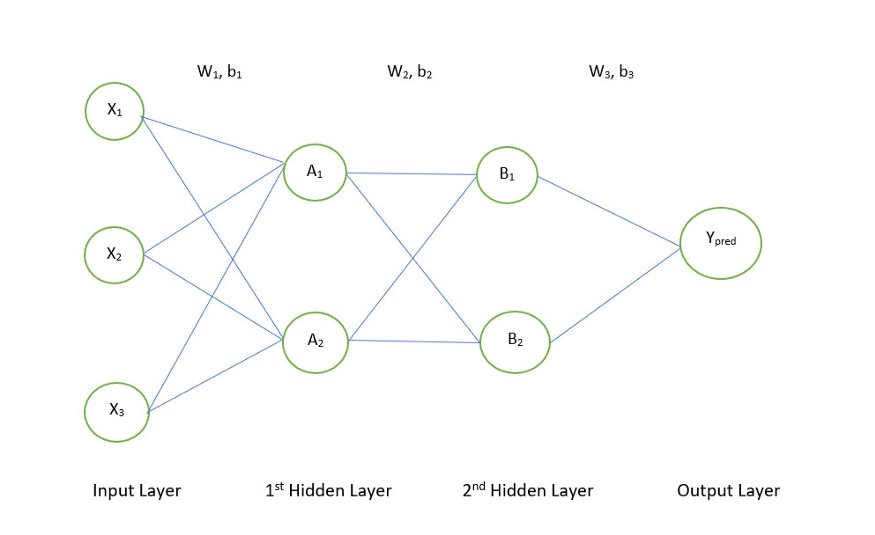
\includegraphics[scale=0.22]{images/neural.jpeg}
    \caption{Neural network \cite{NN_Intro_TB_2020}}
    \label{fig:neuron_img.png}
\end{figure}



\section{Methodology}
%Discuss your research methodology. Did you employ qualitative or quantitative research methods?
%Did you administer a questionnaire or interview people? Any field research conducted? How did you collect data?
%Did you utilize other libraries or archives? And so on. For example, see next paragraph:\\
\indent In this research, we analyze a total of 185 distinct simulated optics patterns from the \emph{Super High Momentum Spectrometer} (SHMS) at Hall C of Jefferson Lab.
There were six different optics correlations  $x_{fp}$ vs. $y_{fp}$  ,  $x_{fp}$ vs. $y^{'}_{fp}$  ,  $x_{fp}$ vs. $x^{'}_{fp}$  ,  $x^{'}_{fp}$ vs. $y_{fp}$  ,  $x^{'}_{fp}$ vs. $y^{'}_{fp}$  ,  $y^{'}_{fp}$ vs. $y_{fp}$  each pattern had 31 optics images with varying optics tunes [Q1, Q2, Q3], corresponding to the spectrometer quadrupole magnets, here summarized in Table \ref{tab:tune_stpSize}:

\begin{table}[h]
	\begin{center}
		\begin{tabular}{llll} % left-aligned, number of l's represent number of headings
                  \hline
                  Quadrupole Magnet & Range & Stepsize \\
                  \hline\hline
	          $Q1$ & [0.945, 1.055] & 0.01  \\
                  $Q2$ & [0.945, 1.055] & 0.01  \\
                  $Q3$ & [0.945, 1.055] & 0.01  \\                       
                  \hline 
		\end{tabular}
	\end{center}
	\caption{Quadrupoles Input Data Details}
	\label{tab:tune_stpSize}
\end{table}


Each of the six 2D SHMS optics pattern correlations were trained separately, using 31 different optics tunes
per correlation plot for a total of 185 images. The optics patters for testing the network consisted of only
varying Q2 from 0.945 to 1.055 in steps of 0.01, while keeping Q1 and Q3 tunes fixed at unity.
To test the neural network after it had been trained, a set of 10 images were used for each 2D optics correlation, where Q1 and Q3
tunes were kept fixed at unity while Q2 was varied from 0.955 to 1.055 in steps of 0.01 for a total of 10 Q2 tunes. Images Data was extracted  \cite{PC_CY_Aug2021} Private communication. C. Yero. August 2021.\\
We had three programs that we used to achieve our goals:
%\begin{itemize}
%    \item \emph{make_2Doptics.C}: This ROOT C++ script reads and loops over ROOTfiles corresponding to specific (Q1,Q2,Q3) settings specified in the actual name of the file being read. Then, for each setting, it reads the relevant leaf variables in the ROOTTree, loops over all entries (events) and fills (per entry) six empty and pre-defined 2D histogram object with the relevant correlated variables. The six 2D correlations are: (xfp\_vs\_yfp), (xfp\_vs\_ypfp), (xfp\_vs\_xpfp), (xpfp\_vs\_yfp), (xpfp\_vs\_ypfp), (ypfp\_vs\_yfp) 

%	The six correlation plots per each (Q1, Q2, Q3) tunes are saved to a ROOTfile of the same name as the input file, but with the extension *\_hist.root
%\end{itemize}
%The Neural network model was designed using Keras library and

%IMPORTANT: Keep explaining what you did, or how was the data collected (I CAN HELP WITH THIS SINCE I WROTE THE CODES TO EXTRACT THE DATA IMAGES)
%(See paragraph below, where I expalined roughly what I actually did. You can write this part as it is, and then put a citation that you got this
%information through me. For example:   (see references.bib in the current directory for bibliography format)

\section{Data Analysis Procedure}

%This is generally the longest part of the paper. It's where the author supports the thesis and builds the argument.
%It contains most of the citations and analysis. This section should focus on a rational development of the thesis with clear
%reasoning and solid argumentation at all points. A clear focus, avoiding meaningless digressions, provides the essential unity
%that characterizes a strong education paper. An example of how to start is in the next paragraph. \\
%This figure position may need to be changed and put someplace else in this file, depending on whether it shows up
%in the location you want in your pdf. (Let me know if you have any issues with the placement of this picture)
\begin{figure}[h]
  \centering
  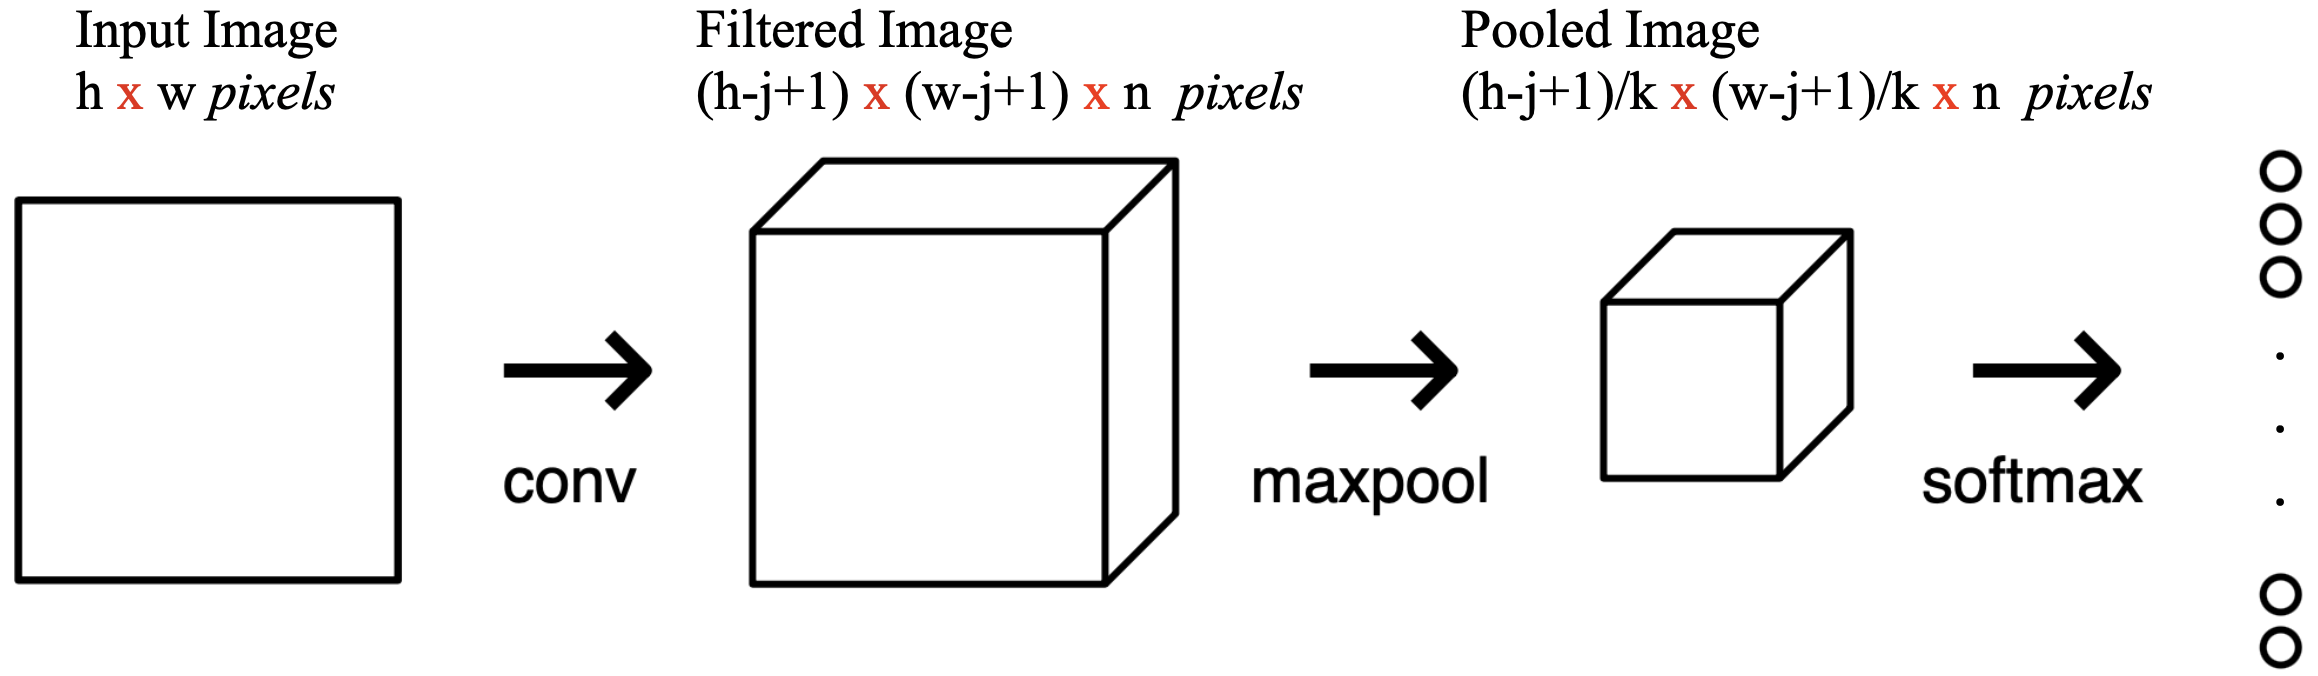
\includegraphics[scale=0.2]{images/CNN_layers.png}
  \caption{CNN layers}
  \label{fig:Layers}
\end{figure}
\indent The Neural Network used in this research consists of 5 layers in total (See Fig.\ref{fig:Layers}). The input and output layers,
represent the raw input image and output model prediction, respectively, and intermediate hidden layers,
\textit{convolutional}, \textit{pooling}, and \textit{activation} layers, each with a specific image analysis task
as described in the subsections below.\cite{CNNPart1_VZ_2019}\\
\subsection{Convolutional Layer}

The convolutional layer is the core building block of a CNN, and it is where the majority of computation occurs. It requires a few components, which are input data, a filter, and a feature map. The feature map will move across the receptive fields of the image, checking if the feature is present. This process is known as a convolution.

\begin{figure}[h]
  \centering
  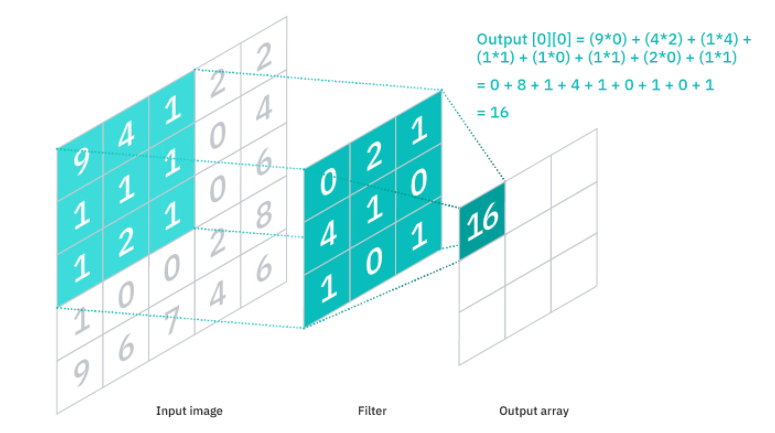
\includegraphics[scale=0.3]{images/conv_demo.png}
  \caption{Convolution Demo\cite{Conv_layer_2020}}
  \label{fig:Conv_demo}
\end{figure}


The feature detector is a two-dimensional \emph{(2-D)} array of weights, which represents part of the image. While they can vary in size, In our case, we are using 1\emph{2} filters of dimension \emph{6x6}. The filter is then applied to an area of the image, and a dot product is calculated between the input pixels and the filter. This dot product is then fed into an output array. Afterwards, the filter shifts by a stride which is 1 in our case, repeating the process until the kernel has swept across the entire image. The final output from the series of dot products from the input and the filter is known as a feature map, activation map, or a convolved feature.

\begin{itemize}
    \item Number of filters: 12
    \item Filter size: 6x6
    \item Stride: 1
\end{itemize}


%Briefly describe what the convolutional layer does, its dimensions, and how many filters used and the filter dimentions. Give reference to the online blog you read, \cite{CNNPart1_VZ_2019}

\emph{Example Figure details Fig.\ref{fig:Convolution}}: 28x28 image is converted to 26x26 to 24x24, with a filter of dimension 3x3 and stride of 1.
\begin{figure}[h]
  \centering
  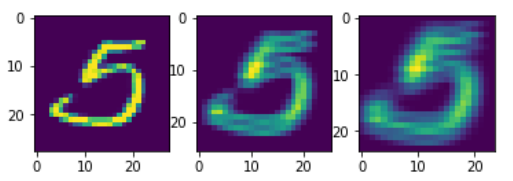
\includegraphics[scale=0.4]{images/conv.png}
  \caption{Convolution\cite{MNIST}}
  \label{fig:Convolution}
\end{figure}



\subsection{Pooling Layer}
Pooling layers are used for dimensionality reduction, to reduce number of parameters. It is similar to convolutional layer, except its output is determined by some aggregation function.

In our case, we used \emph{5x5} MaxPooling, in which filter (5x5) moves across the input, and returns the pixel with largest value to output array.

Although, in pooling layers, lot of information is lost, but it reduces complexity and solves the chances of overfitting.

\emph{Example Figure details Fig.\ref{fig: maxpool}}: 28x28 is converted to 14x14 to 7x7, with 2x2 maxpooling.
\begin{figure}[h]
  \centering
  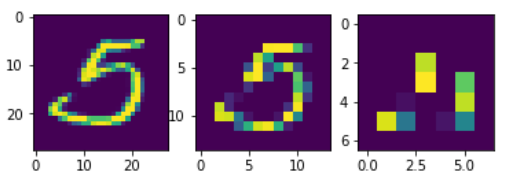
\includegraphics[scale=0.4]{images/maxpool.png}
  \caption{Maxpooling\cite{MNIST}}
  \label{fig: maxpool}
\end{figure}

%Briefly describe what the convolutional layer does, and which specific pooling did you used, e.g., maxpooling?. Give reference to the online blog you read, 
\subsection{Activation Layer}

This layer aims to classify the images on basis of its features of previous layer. In this layer, all the previous layer nodes connect directly to output nodes. In our case we used \emph{Softmax Layer}\cite{CNN_Keras_VZ_SM_2019}, which uses Softmax function for its classification.

We can see in Fig \ref{fig: softmax}, first layer shows outputs from Maxpooling, and it is connected to second layer via a neural network connection, which has certain number of classes, number of classes depends on the number of outputs we want, and then begins the softmax transformation.

\begin{figure}[h]
  \centering
  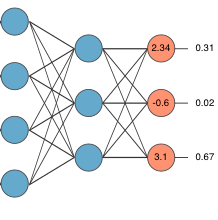
\includegraphics[scale=0.5]{images/softmax_img.png}
  \caption{Softmax\cite{Smax_img_2020}}
  \label{fig: softmax}
\end{figure}

Given a set of numbers, softmax function converts them into probabilities.
Softmax performs the following transform on n numbers \(x_1,\ldots,x_n\)


\begin{equation}
    S(x_n)=\frac{e^{x_i}}{\sum_{j=1}^n e^{x_j}}
\end{equation}


The reason for converting them into probability spectrum is to consider relative chances of being predicted correct, and how much our class' prediction is true than other classes, which helps in training our model. 
The output of these layers are always less than 1 and sums up to 1.

\break

\emph{Cross entropy loss}:
It is calculated by taking the logarithm of correct class' probability.
\begin{equation}
    L = -\ln(p_c)
\end{equation}
\begin{figure}[h]
  \centering
  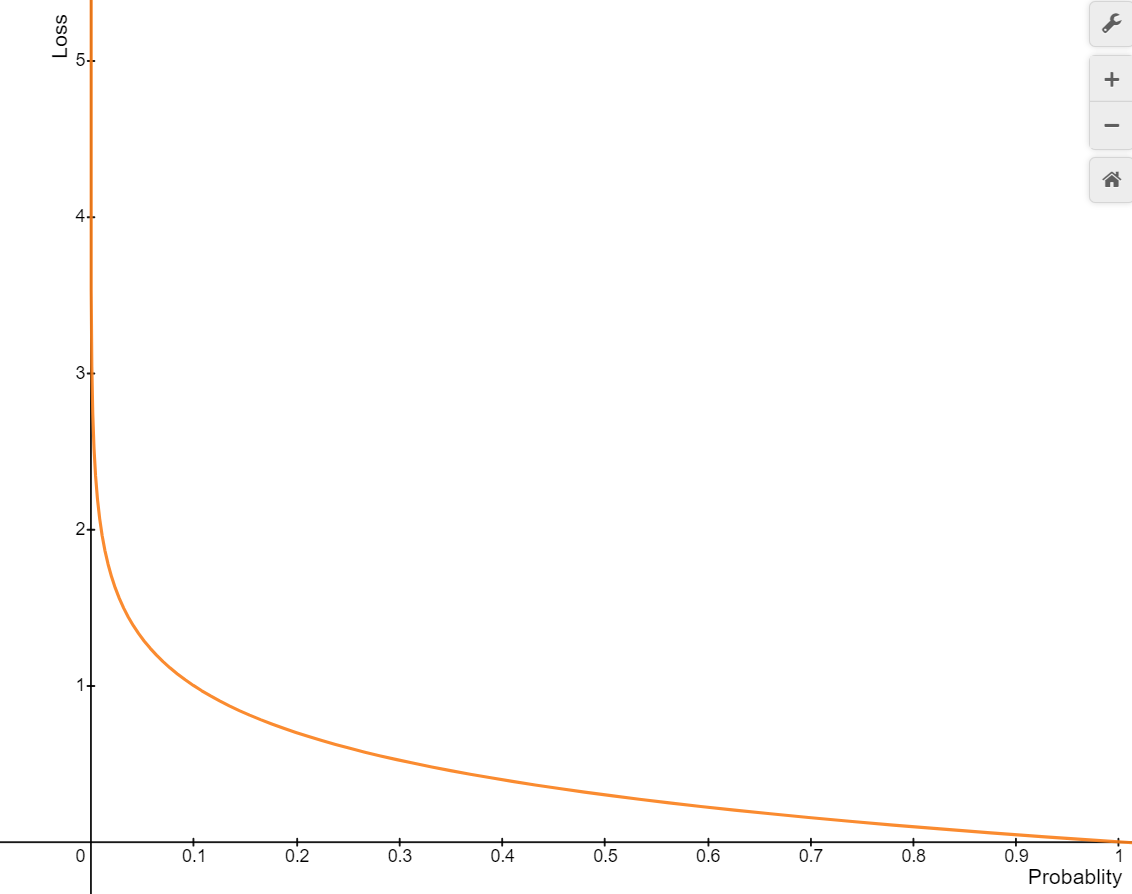
\includegraphics[scale=0.2]{images/Prob_graph.png}
  \caption{Probability Loss graph\cite{Desmos_Oct2021}}
  \label{fig:Probablity graph}
\end{figure}

If probability of correct class is close to one (means our prediction is better) then the loss is close to zero, but if the probability is close to 0 then penalty will be high and loss will approach infinity.



%Briefly describe what the activation layer does, and which specific activation layer did you used, e.g., softmax. Maybe you can put the formula of softmax, and introduce mention how the loss is calculated. If you have not
%talked about what the the loss, then also give a brief description of what it is (See Ref. \cite{}). For the layer description, give reference to the online blog you read, \cite{CNNPart1_VZ_2019}, and probably also
%the article which describes what is softmax. You will need to probably add a new reference to the bibliography to be able to cite the softmax online article, similar to the other citations you have been doing.\\

\emph{Backpropagation}\cite{CNNPart2_VZ_2020}: In forward phase, the inputs of one layer were passed to next layer and completely through the network, whereas in backward phase gradients are backpropagated through the network and weights are updated.

During forward phase, network will store the data like inputs, input size, intermediate values, etc,
and Each layer will receive a gradient of Loss with respect to output. ($\frac{\partial L}{\partial out}$), and will give the gradient of Loss with respect to input ($\frac{\partial L}{\partial in}$). In our case, we are using loss as negative of logarithm of probability of correct class. 

Next step was to update the values of weights and biases, we used the stochastic gradient descent method. In SGD method, all the variables are updated using following equation,
\begin{equation}
x  \longleftarrow x -\alpha \frac{\partial L}{\partial x}
\end{equation}
$\alpha$ is learning rate, It depends on this constant how fast or slow will our loss converge to zero. Overall, x will converge to that value which will result into minimum loss.



%**IMPORTANT:  Don't worry about putting the details of the math (partial derivatives) that was done to actually carry out the forward/bacpropagation of the neural network.
%Just focus on explaining the basics of each layer used, and just mention that once the image passed through the layers, the output was compared to the known result, and
%a backpropagation method was done to minimize the loss by determining the optimum parameters. And mention that an epoch consists of a complete forward/backward propagation.
%Then, the images were re-analyzed with the updated parameters in subsequent epochs to further optimize the parameters and minimize the loss.  ** You'll probably have to also
%give a brief 1-sentence description of what the loss is in a neural network.\\
%\indent The data with specific [Q1,Q2,Q3] tunes were simulated using the standard Hall C simulation program (\texttt{mc-single-arm})
%and the raw data output was written to a ROOTfile. A separate ROOT C++ script (\texttt{make\_2Doptics.C}) was used to form each of
%the six abovementioned 2D focal plane correlations correlations which were stored in a separate ROOTfile as histogram objects.
%The 2D histograms were then converted to a 2D pixelated array and stored in binary format (.h5) via a Python code (\texttt{save2binary.py})
%array to be read by the Neural Network using Python Keras. Each optics image used was 200x200 pixels and was passed thorugh each of
%the hidden layers of the network described in Section 4 of this article.

\break

Figure \ref{fig: layers} illustrates the transformations on our image,
From 200x200x12 to 195x195x12 to 49x49x12 to 1x10.

\begin{figure}[h]
  \centering
  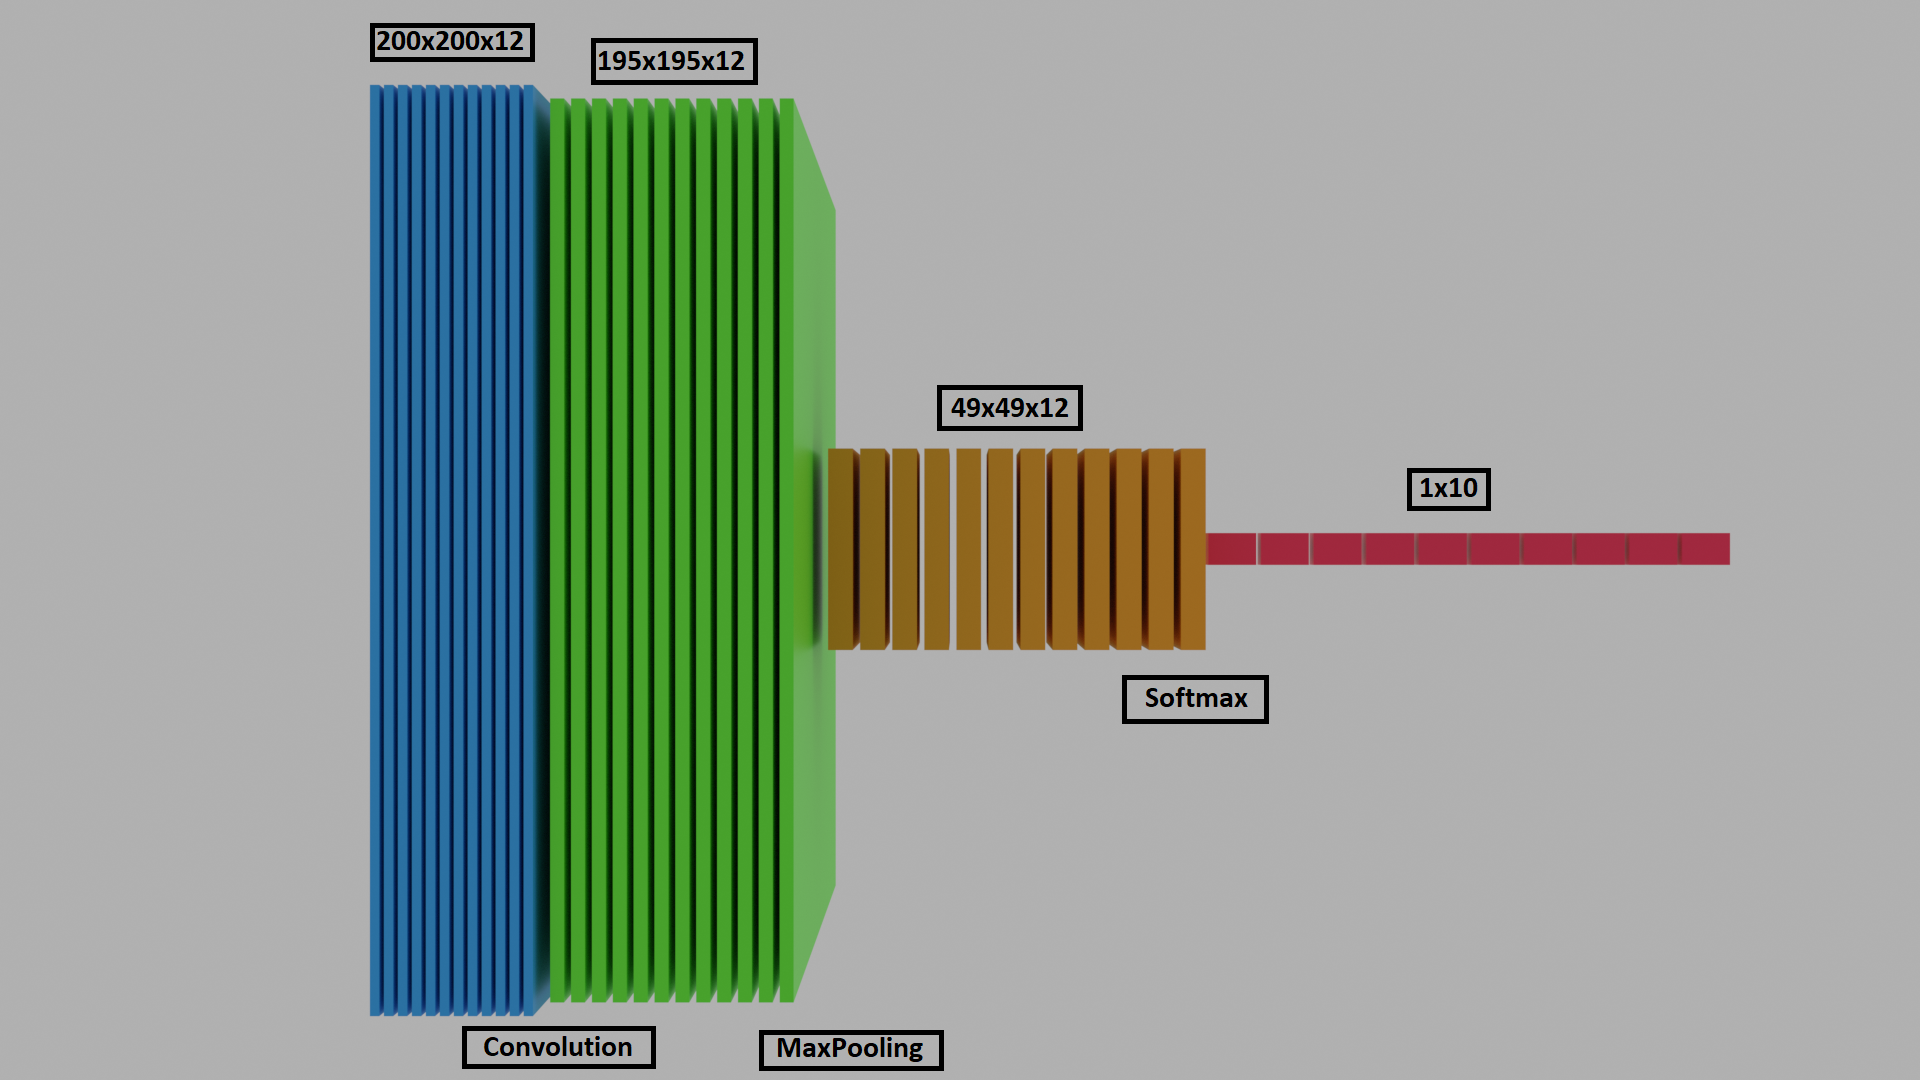
\includegraphics[scale=0.2]{images/layers_image.png}
  \caption{Layers in our network\cite{Blender_Aug2021}}
  \label{fig: layers}
\end{figure}




\section{Results and Discussion}
%Summarize results and discuss implications of these results. After spending a great deal of time and energy introducing and arguing the points in the main body of the paper,
%the conclusion brings everything together and underscores what it all means. A stimulating and informative conclusion
%leaves the reader informed and well-satisfied. A conclusion that makes sense, when read independently from the rest of
%the paper, will win praise. \\
\indent The purpose of this research was to teach a machine to recognize optics patterns that would otherwise be
difficult to distinguish by the "human eye". With the help of Keras API, we were able to train and test a CNN
by providing simulated optics data from Jefferson Lab, Hall C.  Each of the six 2D optics correlation was trained with
31 optics tunes, and each were able to reach and plateau at an accuracy of ~100 \%, and a average loss of ~0.3787 , in 100 epochs of training.
We used 10 test images per each of the six 2D optics correlations, and network was able to correctly predict each of the patterns with average of ~80\% accuracy. The results of the training are shown in Fig.\ref{fig: epochs graph1} and Fig.\ref{fig: epochs graph2}

\begin{itemize}
\item \emph{Result: Accuracy vs Epochs}: In training graph \ref{fig: epochs graph1}, we can see that till 100 epochs all the correlations have achieved 100 \% accuracy.
\item \emph{Result: Loss vs Epochs}: Similarly, graph \ref{fig: epochs graph2} tells us that loss is approaching $0$.
\end{itemize} 

\begin{figure}[h]
  \centering
  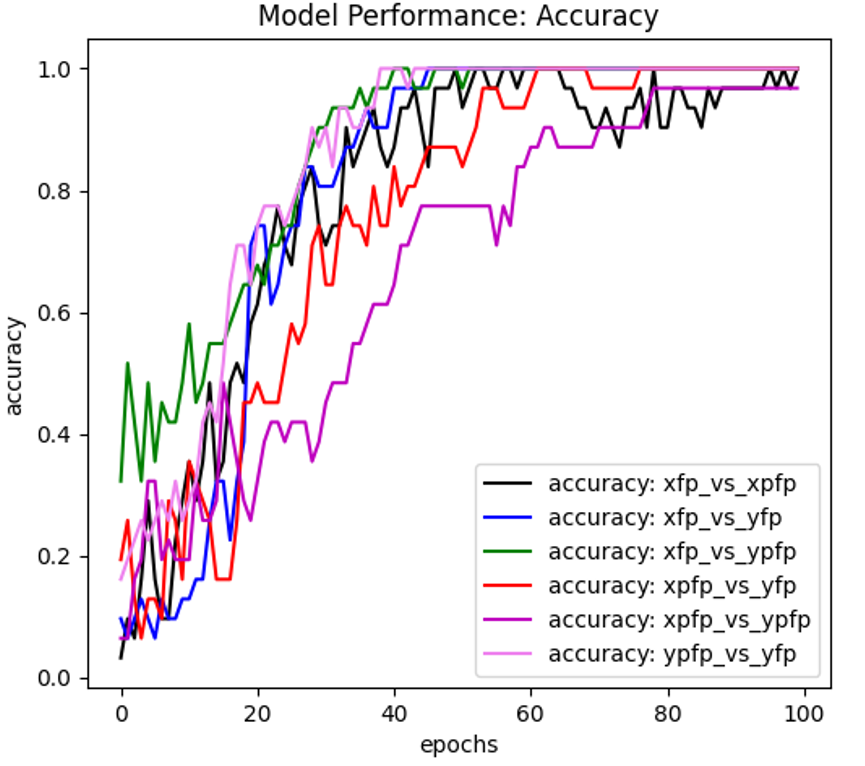
\includegraphics[scale=0.29]{images/acc_plot.png}
  \caption{Accuracy vs epochs plot}
  \label{fig: epochs graph1}
\end{figure}

\begin{figure}[h]
  \centering
  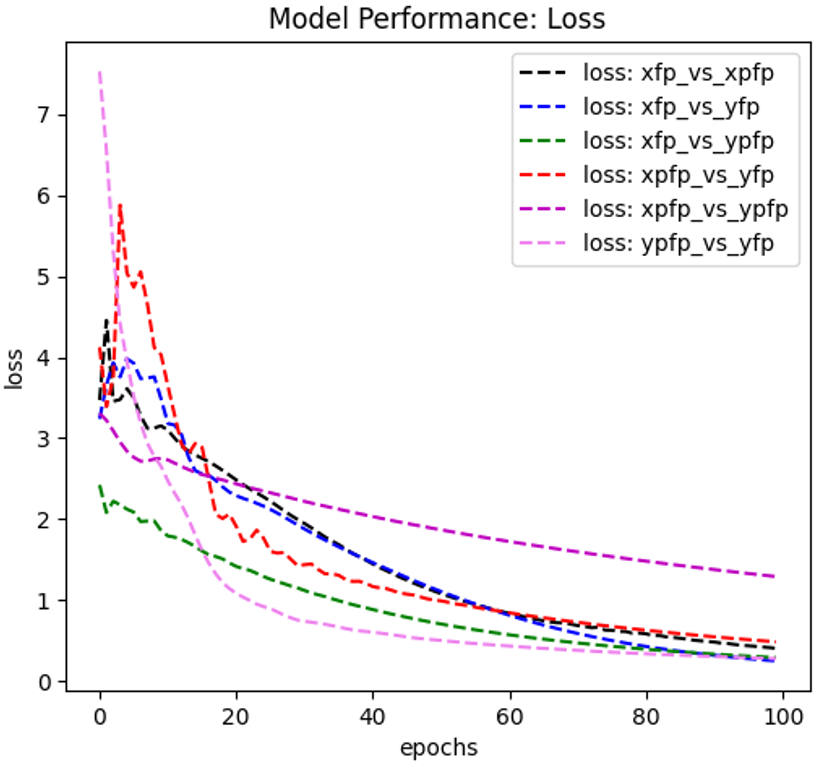
\includegraphics[scale=0.3]{images/loss_plot.png}
  \caption{Loss vs epochs plot}
  \label{fig: epochs graph2}
\end{figure}


The results of the test images is summarized in Table \ref{tab:results}
\begin{table}[h]
	\begin{center}
		\begin{tabular}{llll} % left-aligned, number of l's represent number of headings
                  \hline
                  2D optics correlation   &  Correct predicted patterns &  No. patterns  & Accuracy \\ \hline \hline
                  $x_{fp}$ vs. $x^{'}_{fp}$  &  8  &  10  &  0.8\\
                  $x_{fp}$ vs. $y_{fp}$  &  8  &  10  &  0.8\\
                  $x_{fp}$ vs. $y^{'}_{fp}$  &  10  &  10  &  1.0\\
                  $x^{'}_{fp}$ vs. $y_{fp}$  &  5  &  10  &  0.5\\
                  $x^{'}_{fp}$ vs. $y^{'}_{fp}$  &  10  &  10  &  1.0\\
                  $y^{'}_{fp}$ vs. $y_{fp}$  &  7  &  10  &  0.7\\
		  \hline
		\end{tabular}
	\end{center}
	\caption{Caption of table.}
	\label{tab:results}
\end{table}

\begin{figure*}[h]
  \centering
  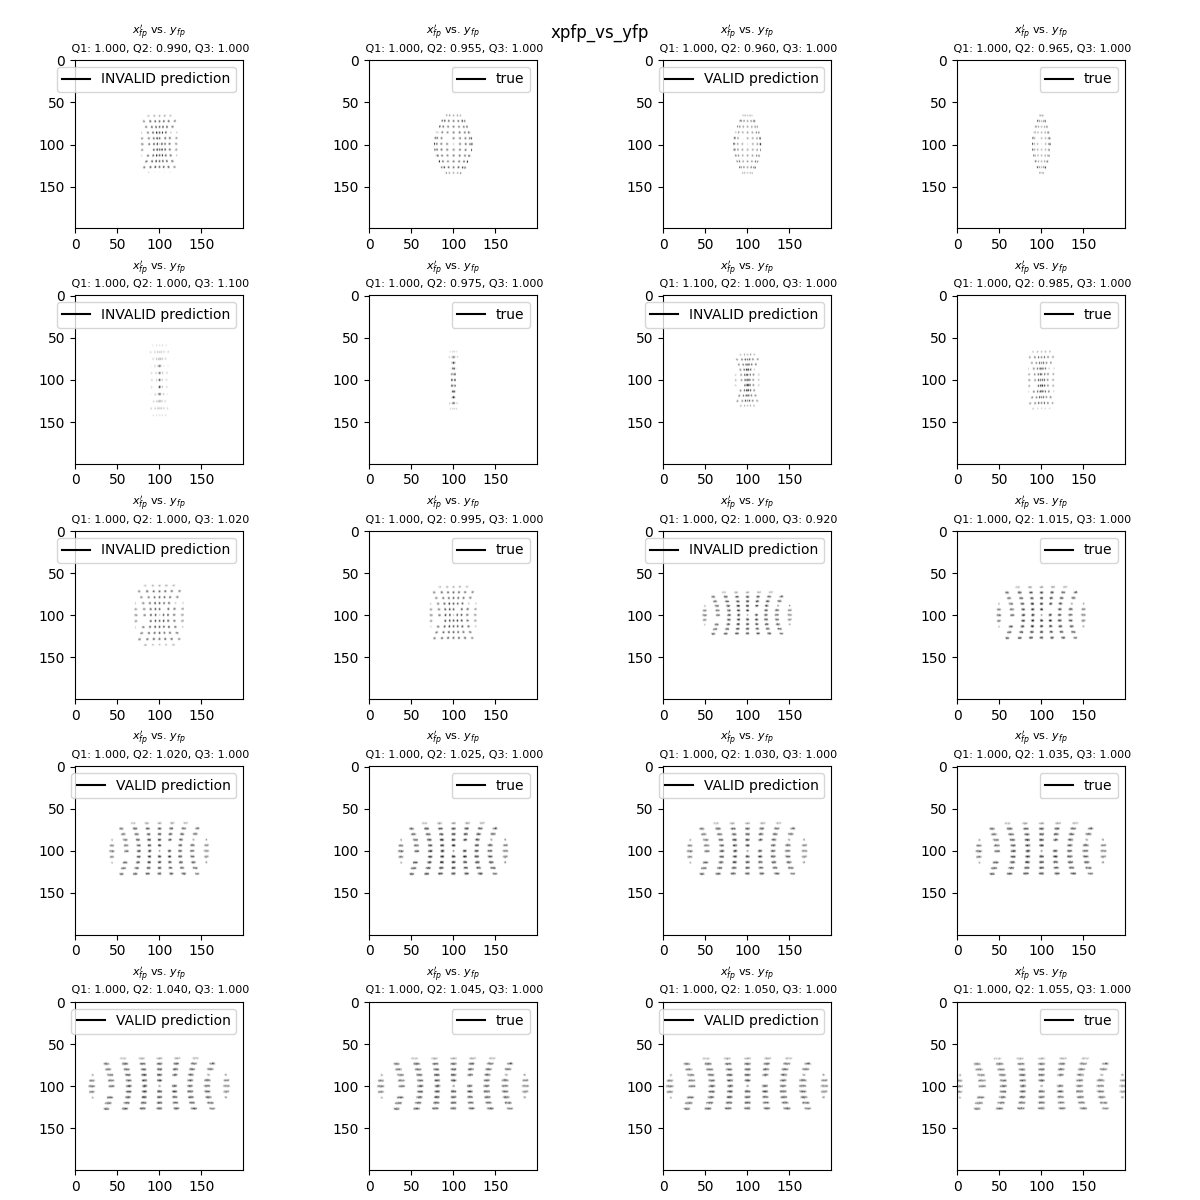
\includegraphics[scale=0.6]{images/final_results_xpfp_vs_yfp.png}
  \caption{xpfp vs yfp: A sample result: clearly we can see that it cannot be distinguished by naked eye. More images can be found in \cite{Result_images}}
  \label{fig: images and their predicted images}
\end{figure*}



\break
\bibliography{references}   
\bibliographystyle{IEEEtran}



\end{document}
